\chapter{Maze complexity problems}\label{cha:background}
One of the main purpose of this paper is to discuss complexity of a maze. This chapter will provide a variety of maze and graph complexity definitions. I will start by reviewing complexity measurement methods derived from graph theory. 
Then I will try to review some existing concept of measuring the complexity of a maze.
I will also try to provide an answer to the question of why is it important to define what complexity means and the implication of such a definition. Thinking about a maze and its complexity, we may think about all different features. 
It may be the difficulty of finding the way out, or difficulty of moving from point A to point B, or difficulty of generating a particular maze. This chapter will provide a theoretical background of studying the maze complexity and in chapter 5 I will provide a detailed analysis based on examples. 
\section{Complexity measures in Graph Theory}
In the below part, I will present the approaches derived from graph theory, which describe and measure the complexity of a graph.
 Conventionally, graph complexity in graph theory is evaluated by degree distribution, clustering coefficient, edge density, community. Another approach which derived from classical information theory is to generate graphs with some particularities while being random in all other aspects and then compare and decide whether a particular characteristic is typical among group of graphs or not.
There is also a recent, advanced idea to use a \textit{principle of maximum entropy} or \textit{maxent} to estimate the algorithmic complexity of a graph. The main idea of maximum entropy concept is that the more statistically random graph is the more typical. \cite{HeZeni}. 
Studying the complexity of a graph is an important part of understanding it. By studying the complexity, we are acquiring knowledge about the system, how it could evolve, what are bottlenecks and variabilities, and how we can solve the problems posed by the system. Each application may understand the complexity differently. 
Each graph system, network and maze will cause different challenges and solutions to it. 
\subsection{Outlining Graph Parameters}
\begin{definition}\textbf{A Degree Distribution} is defined as a proportion of vertex with a degree $k$ to all vertices in a graph.
\begin{equation}
P(k) = \frac{n_k}{n}
\end{equation}
\end{definition}
\begin{definition}\textbf{A Clustering Coeficient} $C_i$ is defined as a proportion of vertex links to vertex possible links. The coefficient for an undirected graph might be given by $C_i = \frac{k_i(k_i-1)}{2}$ where $k_i$ are the neighbours of vertex $v_i$. The average clustering coefficient is given by
\begin{equation}
\bar{C} = \frac{1}{n}\sum_{n = 1}^{n} C_i
\end{equation}
\end{definition}
\begin{definition}\textbf{A Community} is a subset of vertices densely connected respectively, and loosely connected to vertices in other communities in the same graph.\end{definition}
\begin{definition}\textbf{A Graph Entropy} “Graph entropy represents information-theoretic measures for characterizing networks quantitatively”\cite{MaDehm}. It is the most important and difficult method to determine graph complexity. There is no “good enough” definition of graph entropy which could be applied to all different kinds of problems. Searching new ways of calculating the entropy of the graph systems is a huge challenge for a scientist from mathematics, physics, biology, chemistry, computer and sociology sciences. We can distinguish 3 major fields of graph entropy: The Classical Entropy, The Deterministic Entropy and The Probabilistic Entropy. All three have different application, sometimes specific. As a result, I will not try to make here a general definition of graph entropy, instead in the next subsection I will provide some more details about Shannon’s entropy measure which is one of the simplest method and I will use it later to calculate maze complexity. \end{definition}
\subsection{Shannon Entropy}
Shanon entropy derives directly from Boltzmann entropy in thermodynamics. “Shannon’s concept of information entropy quantifies the average number of bits needed to store or communicate a message.”\cite{HeZeni}. Studying complexity, the Shannon entropy measures how complex the string of a graph problem must be to avoid losing any information about its state. The main concept is that the information is built by $n$ different symbols and can not be stored in less than $log(n)$ bits.
Shanon entropy of the object $M(R, p(x_i))$ is given by (1.3)\cite{HeZeni}:

\begin{equation}
H(M) = - \sum_{n = 1}^{n} p(x_i)\log_2 p(x_i)
\end{equation}
\textbf{Where:}\\
$R$ is a set of possible outcomes, e.g.  All possible adjacency matrix of size $m$\\
$p(x_i)$ is a probability of outcome $R$,\\
$n= |R|$\\
\section{Maze Complexity Measures}
In this section, I will discuss the characteristics which impacts the complexity of a maze. I will try to make an overview of different approaches and try to compare them. Since the problem of maze complexity isn’t well described in the literature, one of the main aim of this work is to provide a complex description of different measures and approaches while exploring a maze complexity problem. 
\subsection{Independant Maze Parameters}
\begin{description}[style=unboxed]
\item[Size] One of the most indisputable complexity factors is the size of a maze. In this work, we use a definition of a maze, which is represented as a square grid, which size is denoted by $s_m = n \times m$. It is almost too easy to think that a small maze is a simple maze, and a huge maze is a difficult one.
\begin{figure}[!h]
    \centering
    \begin{subfigure}{.5\textwidth}
    \centering
    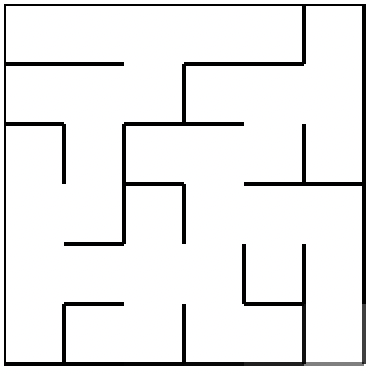
\includegraphics[width=.5\linewidth]{66}
    \caption{An Aldous-Broder maze size $6 \times 6$}
\label{fig:sub1}
    \end{subfigure}%
    \begin{subfigure}{.5\textwidth}
    \centering
    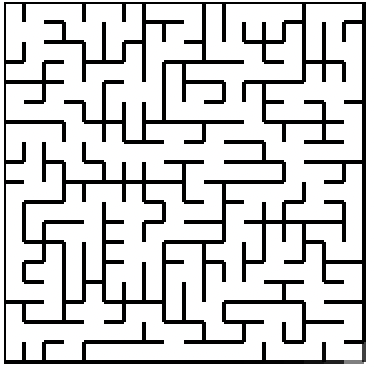
\includegraphics[width=.5\linewidth]{1818}
    \caption{An Aldous-Broder maze size $18 \times 18$}
\label{fig:sub2}
    \end{subfigure}
    \caption{Examples of different size mazes}
\label{fig:test}
\end{figure}
\item[Path length] Another key characteristic determining the complexity of a maze is the average length $\bar{p_l}$ of the paths. The longer the path, the bigger the risk of following a faulty road to a solution. I consider a path in this case as a sequence of moves from the start to each dead-end in acyclic mazes. In cyclic mazes, paths can be infinite.
\newline

\begin{figure}[!h]
\centering
\begin{subfigure}{.5\textwidth}
\centering
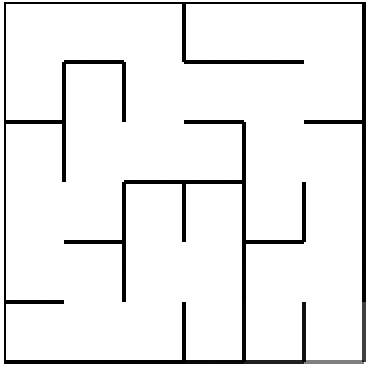
\includegraphics[width=.5\linewidth]{aldous}
\caption{An Aldous-Broder maze with $\bar{p}_l = 9.42$}
\label{fig:sub1}
\end{subfigure}%
\begin{subfigure}{.5\textwidth}
\centering
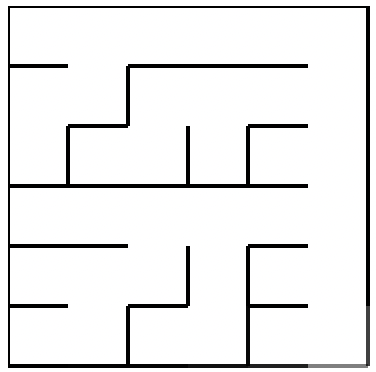
\includegraphics[width=.5\linewidth]{binary}
\caption{A Binary Tree maze with $\bar{p}_l = 10.8$}
\label{fig:sub2}
\end{subfigure}
\caption{Examples of different average path length mazes}
\label{fig:test}
\end{figure}

\item[Density] Density for an acyclic graph is given by (\ref{acyclic_density}), and density for cyclic maze is given by (\ref{cyclic_density})\cite{SBorg}. It describes the ratio between the number of all possible connections and the existing number of connections ( edges)
\begin{figure}[!h]
\centering
\begin{subfigure}{.5\textwidth}
\centering
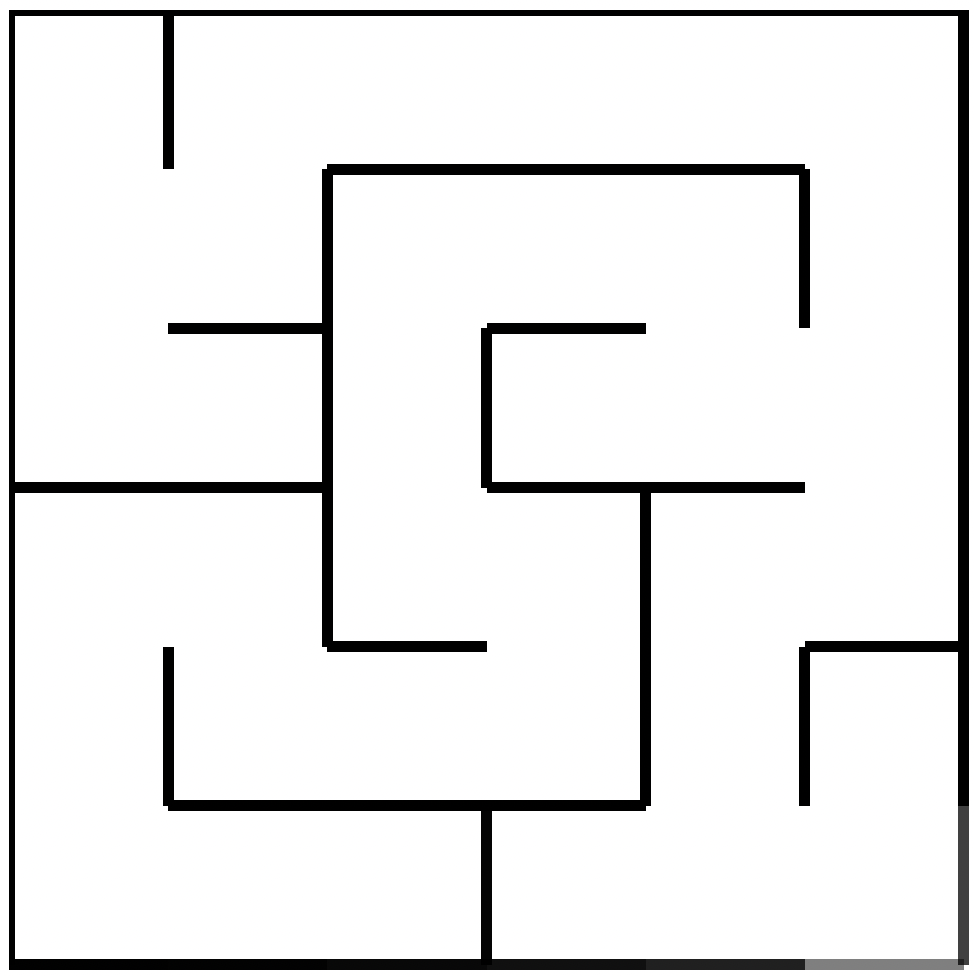
\includegraphics[width=.5\linewidth]{recursivedens}
\caption{A recursive-backtracker maze with $density = 0.40$}
\label{fig:sub1}
\end{subfigure}%
\begin{subfigure}{.5\textwidth}
\centering
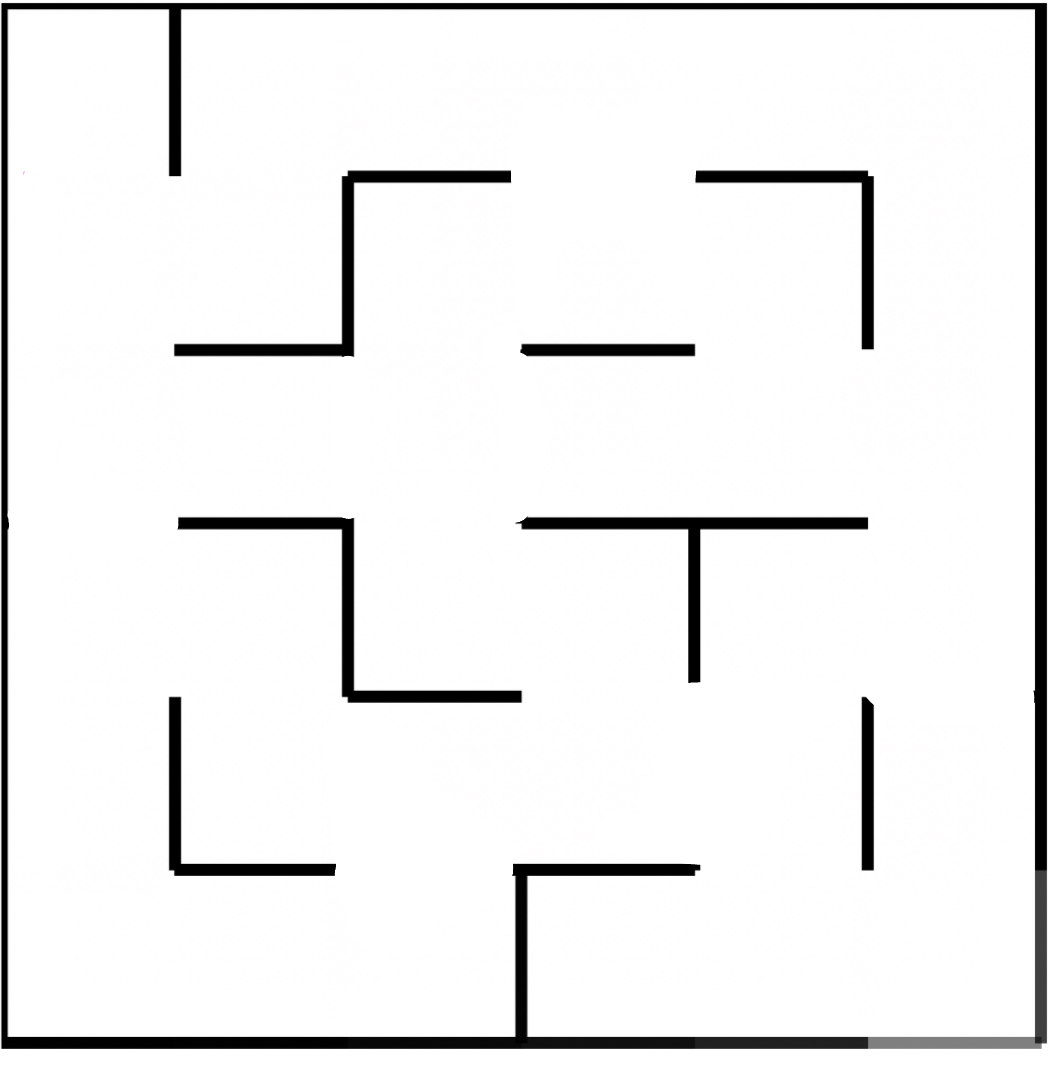
\includegraphics[width=.5\linewidth]{recursivedensecyclic}
\caption{A Binary Tree maze with $density = 0.50$}
\label{fig:sub2}
\end{subfigure}
\caption{Examples of different density mazes}
\label{fig:test}
\end{figure}
\end{description}
\newpage
\subsection{McClendon Measure}
There are few sources indicating a quantitative study of the measure of maze complexity. One of the most cited work in this field is a McClendon study of maze difficulty and complexity. 
McClendon’s work treats about maze complexity and difficulty in continuous measure using continuum theory. Main presuppositions of the work are that the maze is a perfect maze type and there are two distinguished pairs of points $(p,q)$ in the maze $M$ called gates. Where $p$ is an entrance and $q$ is an exit.  Hallways  $h$ build a maze. 
Where hallways are a subset $K$ of $M$ with the $degree = 2$. A subset $W_h = {w_1,w_2,\ldots, w_n}$ of $h$ incorporates all points of $h$. 
A trail is a path in the maze build by hallways. The branch is any trail intersecting the solution $T$ of a maze. Each branch in $M$ is connected to $T$ by a point $v_i$ in $I$ which is an intersections set $I = {v_1,v_2,\dots, v_n}$. The McClendon’s complexity of a hallway $h$ is given by:\\
\begin{equation}
\gamma(h) = D(h)\sum_{n = 1}^{n} \frac{\theta(w_i)}{d(w_i)\cdot \pi}
\end{equation}
\textbf{Where:}\\
 $D(h)$ is an arclength of $h$,\\ 
$\theta(w_i)$ is the absolute value of the difference in the radian measures between the directions $V(t_i)$ and $V(t_{t+1})$\\ 
$d(w_i)$ is a length of a arc between $w_{i-1}$ and $w_i$ in $W_h$.\\ 
\newline
The McClendon’s complexity of a Maze $M$ is given by:\\
\begin{equation}
\gamma(M)=\log\bigl[\gamma(T) + \sum_{n = 1}^{n} \gamma(B_i) \bigr]
\end{equation}
\textbf{Where:}\\
$\gamma(T)$ is a complexity of a solution of the maze\\,
$\gamma(B_i) = \sum_{n = 1}^{n} \gamma(h_i)$ is a complexity of a branch $B_i$.\\
\newline 
In the method above to calculate the complexity of a maze, we must know the solution of the maze. To avoid this, we should use the extrinsic approximation of the above method which is given by:\\
\begin{equation}
\gamma(M) \approx \log \bigl[\sum_{n =1}^{n}\gamma(h_i)\bigr]
\end{equation}
\\
\textbf{Where:}\\
$y(h_i)$ is the complexity of $h_i$\\
 \newline
In this paper we are using the square grid to generate and solve mazes. As a result of uniform grid, the McClendon measure will be simplified, and calculated as:
\begin{equation} 
\gamma(M) \approx \log \bigl[\sum_{n =1}^{n}\frac{h(i)_l\cdot \mathcal{T}}{2}\bigr]
\end{equation}

\textbf{Where:}\\
$h(i)_l$ is the total length of the hallway,\\
$\mathcal{T}$ is the total number of L turns in the hallway, and each L turn is 90$^\circ$.%porownac to co wyjdzie z tym wykresem w tej pracy 
\subsection{Other approaches to delineate maze complexity }
In sections above we discussed different quantitative measures to define maze complexity. But we can also list at least two  descriptive methods determining the difficulty of the maze.\\ \newline
\textbf{Time Complexity of maze generators}\\
Looking at time complexity of maze generators we can compare them and  analyze whether the solution time depends on the time complexity. Below in Table 1.1 time complexity of different maze generator is presented. The analysis of the relation between time complexity and solution time is presented in Chapter 5.\\
\begin{table}[!h]
\begin{center} 
\begin{tabular}{ |p{6cm}||p{3cm}| } 
\hline Maze Generator Algorithm Name& Time Complexity\\ \hline Binary Tree & $O(|V|)$\\ Aldous-Broder& $O(|V|^3)$ \\ 
Recursive- Backtracker& $O(|V|+|E|)$\\ 
\hline
 \end{tabular} 
\caption{\label{tab:table-name}Time complexity of maze generating algorithms.} 
\end{center}
 \end{table}
 \newline
\textbf{Uniquness and Distinctivness of a Maze}\\
Another approach of describing a maze might be evaluating it uniqueness and distinctivens. For this purpose, it is possible to study how complicated the algorithm generating a given maze must be and how statistically often a specific set of features occurs. One of the methods may be the parameterization of the maze by classic measures as density distribution or average path length and testing how often they appear in a specific configuration. Another method could be to look for biased features. Biased features are some peculiarities of the maze which are visible repeating structures.
Good examples of biased maze might be a binary tree algorithm, which tends to create a visible diagonal intersections, and two perpendicular corridors at the edges of the maze. The texture of maze is visible after applying coloring see Figure (1.4). The colors represent the distance from starting point. 

\begin{figure}[!h]
    \centering
    \begin{subfigure}{.7\textwidth}
    \centering
    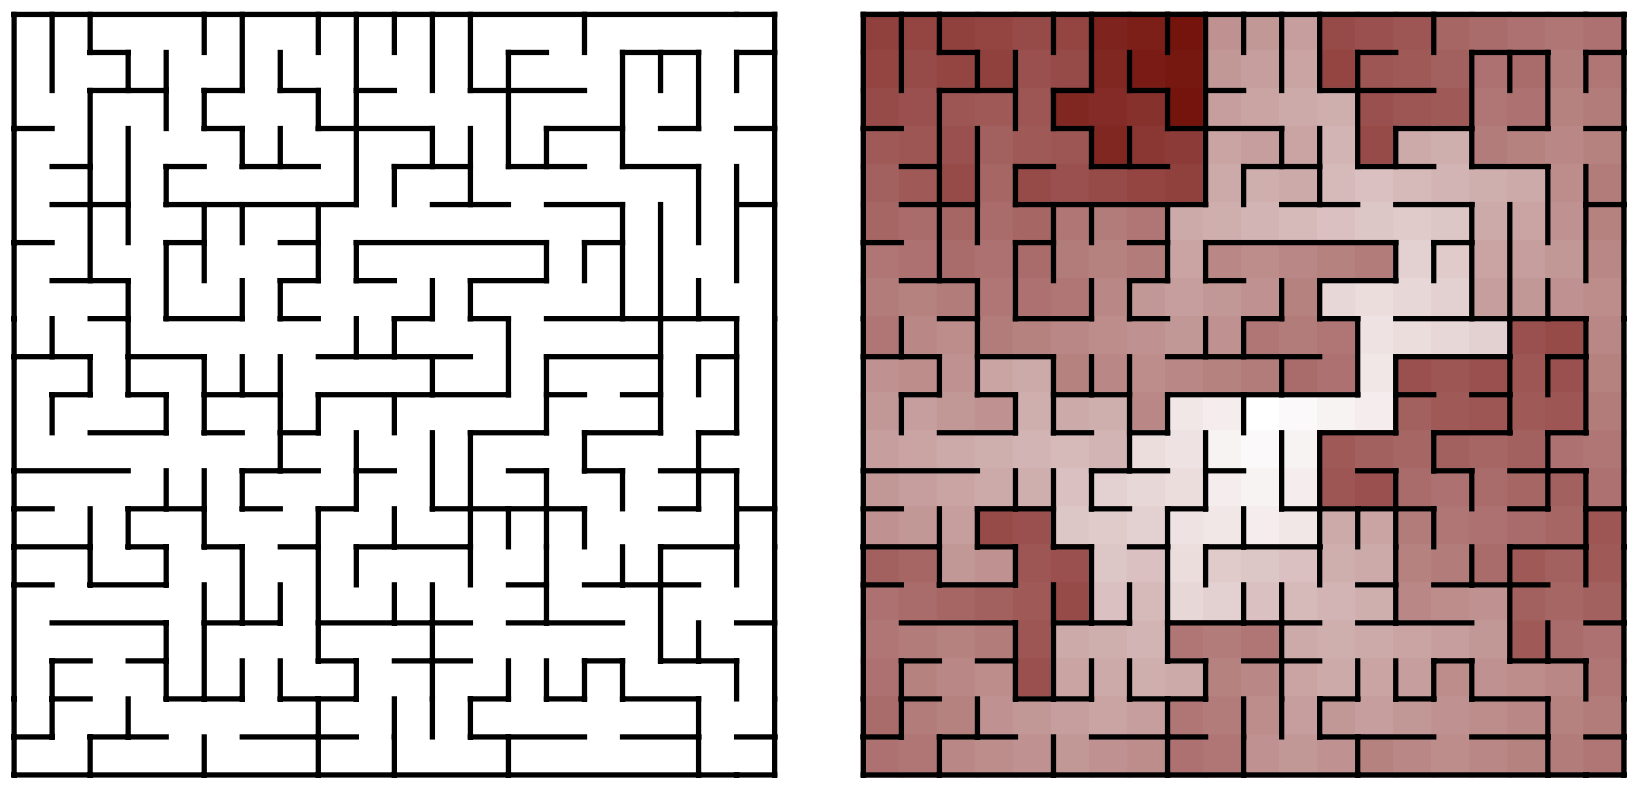
\includegraphics[width=.7\linewidth]{adlousbias}
    \caption{An example of non-biased maze generated by Aldous-Broder algorithm. Figure comes from \cite{JaBuck}.}
    \label{fig:sub1}
    \end{subfigure}%

    \begin{subfigure}{.7\textwidth}
    \centering
    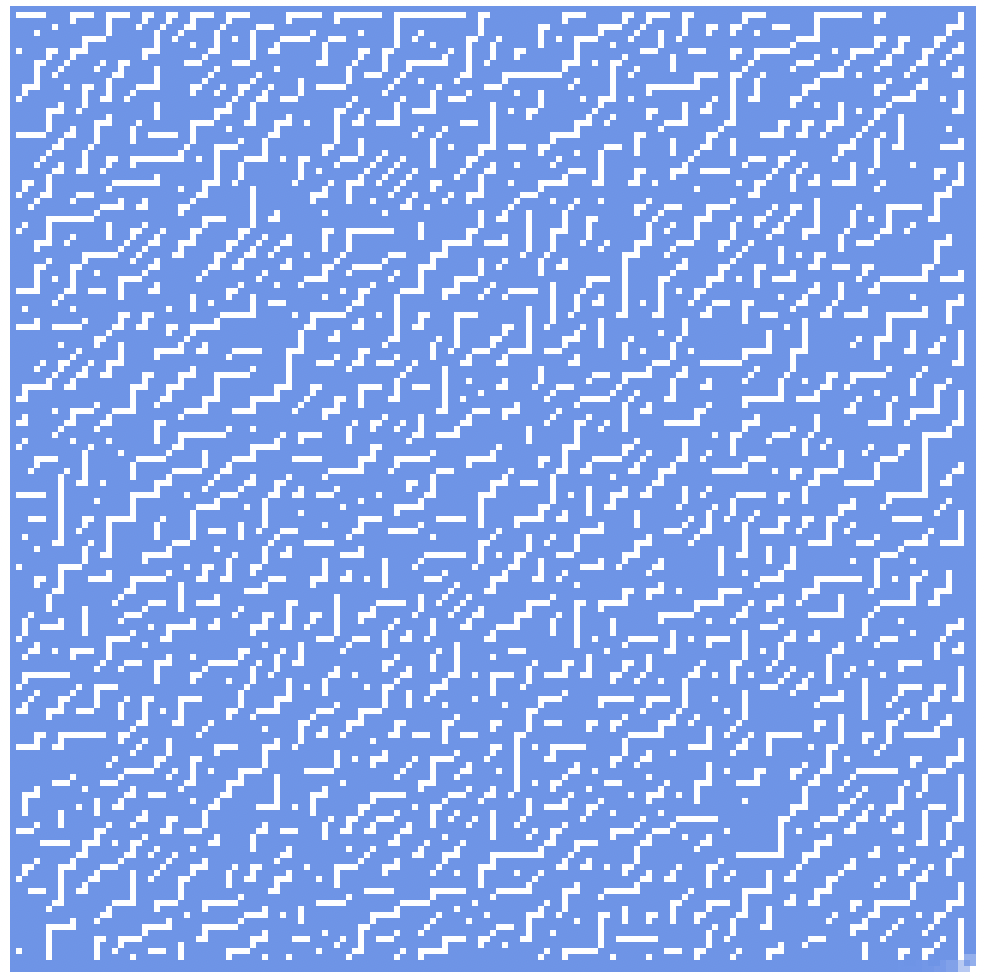
\includegraphics[width=.7\linewidth]{binarybias}
    \caption{An example of biased maze generated by Binary Tree algorithm. Figure comes from \cite{JaBuck}.}
    \label{fig:sub2}
    \end{subfigure}
    \caption{Examples of different maze tectures.}
    \label{fig:test}
    \end{figure}


 %typical path lenght
 %człowiek a komputer
 %how many visited cells during solution
 %zgodny z heurystyką